\documentclass[sigconf]{acmart}

\usepackage{booktabs} % For formal tables

\settopmatter{printacmref=false} % Removes citation information below abstract
\renewcommand\footnotetextcopyrightpermission[1]{} % removes footnote with conference information in first column
\pagestyle{plain} % removes running headers

\begin{document}

\title{Automated Sharded MongoDB Deployment and Benchmarking for Big Data Analysis}

\author{Mark McCombe, Gregor von Laszewski, Geoffrey C. Fox}
\affiliation{%
  \institution{Indiana University, Smith Research Center, 2805 E 10th
    St, Bloomington, Indiana, 47408}
}
\email{laszewski@gmail.com}


\begin{abstract}
  Project CH-818664, KVM: 
Using Python, Ansible, Bash Shell, and Cloudmesh Client a fully
automated process is created for deploying a configurable MongoDB
sharded cluster on Chameleon, FutureSystems, and Jetstream cloud
computing environments.  A user runs a single Python program which
configures and deploys the environment based on parameters specified
for numbers of Config Server Replicas, Mongos Instances, Shards, and
Shard Replication.  The process installs either MongoDB version 3.4 or
3.2 as requested by the user.  Additionally, functionality exists to
run benchmarking tests for each deployment, capturing statistics in a
file as input for python visualization programs, the results of which
are displayed in this report.  These reports depict the impact of
MongoDB version and degrees of sharding and replication on
performance. Key performance findings regarding version, sharding, and
replication are abstracted from this analysis.  As background,
technologies and concepts key to the deployment and benchmarking, such
as MongoDB, Python, Ansible, Cloudmesh Client, and Openstack are
examined while comparing and using them within different clouds.
\end{abstract}

\keywords{Chameleon CLoud, Jetstream, Futuresystems, MongoDB, Cloud
  Computing, Ansible, Python, Cloudmesh Client, Openstack}


\maketitle

\section{Introduction}


Three clouds were selected for deployment: Chameleon Cloud,
Futuresystems (also referred to as Kilo in some sections of this
document), and Jetstream.  In our automated deployment and
benchmarking process, the cloud name is passed as a parameter to the
deploy function of the main script and a customized version
of MongoDB is deployed to the selected cloud.



\section{Cloud Usage}

We compared within the allocation limitations of a class multiple
cloud performances by varying a number of parameters.  In addition to
Chameleon cloud we also used Jetstream and the Futuresystems
cloud. Adding these clouds was essential to obtain comparisons of
chameleon cloud to other clouds.  A full report is available as part
of the Class proceedings.

Table \ref{tab:cloud-comparison} shows a comparison of key server computing
resources on Chameleon, FutureSystems, and Jetstream cloud
environments.

\begin{table}[htbp]
\centering
\caption{\bf Cloud Server Hardware Specification Comparison \cite{www-chamHardware} \cite{www-kiloHardware} \cite{www-jetHardware}}

 \begin{tabular} {| c | c | c | c |}
\hline
  & FutureSystems &  Chameleon  & Jetstream \\ [0.5ex] 
 \hline

    
CPU     &     Xeon E5-2670 & Xeon X5550 & Haswell E-2680  \\
 \hline
cores &  1024             &        1008   &  7680 \\
 \hline
speed     &   2.66GHz           &               2.3GHz & 2.5GHz\\
 \hline
RAM   &     3072GB            &               5376GB  &  40TBr\\
 \hline
storage     &     335TB     &                   2TB  & 2 TB\\ [1ex] 
 \hline

\end{tabular}
  \label{tab:cloud-comparison}
\end{table}


\section{Projects}


\section{Experimental configuration}

Cloudmesh client is used to simplify management of vms accross
different clouds.  The Cloudmesh Client toolkit is an open source
client interface that standardizes access to various clouds, clusters,
and workstations \cite{www-cloudmesh}.  Cloudmesh Client is a python
based application. In the deployment, Cloudmesh Client is used to
handle most interaction with the Virtual Machines in the
clouds. Cloudmesh Client provides functionality in three main areas:
Key Management, OpenStack Security, and virtual machine management.
For key management, Cloudmesh's key add and upload commands simplify
secure interaction with the cloud environments.  For Openstack
security, Cloudmesh's secgroup commands allow new security rules to be
added and uploaded to the cloud.  Virtual machine management is
performed with Cloudmesh's cluster functionality, which allows easy
creation and deletion of virtual machines and communication between
them.  Cloudmesh Client simplifies and standardized interaction with
the cloud for these tasks.  This allows us to more easily port the
deployment to additional clouds that are supported by Cloudmesh.
Furthermore, by encapsulating the logic necessary to perform these
tasks we are shielded from changes in interfaces made by individual
clouds.

\subsection{Resource Requirements}

As this project was a class project the available VM hours were
limited, HOwever we have been able to conduct a significant
comparision given the restrictions.

\subsection{Capability Requirements}

The main feture we needed for this project was the creation of VMs and
the execution of our applications within these VMs

\subsection{Monitoring Requirements}

Monitoring and benchmarking was conducted by hand without need for
specialized services. 

\subsection{Features offered by Chameleon Cloud}

Chameleon provided one of three clouds to the project.


\subsection{New software created}

As part of this class we improved the cloudmesh client software
\cite{www-cloudmesh-client}\cite{www-cloudmesh-cmd5}
\cite{www-cloudmesh-rest} that was essential to the success of the
class.

\subsection{Performance Comparison}

We have conducted a significant performance comparision among all
clouds. However in thsis document we only list a few highlights.

\subsection{Computing Resources}

In all cases, virtual machines are deployed with the Ubuntu 16.04 LTS
(Xenial Xerus) operating system.  On Openstack the flavor or the
machine determines the amount of computing resources (CPU, memory,
storage) allocated to it.  In our testing, m1.medium was used as the
flavor for Chameleon Cloud and FutureSystems, while  m1.small was used
on Jetstream.  Jetstream has more resources allocated to each flavor
than Chameleon and FutureSystems, which are similar.  In order to
perform similar tests on each cloud, flavors with identical CPU and
memory were selected. Table \ref{tab:computing-resources} shows the
comparative resources of the flavors used in our testing.  While
storage is lower on Jetstream, it is sufficient for out tests and
should not significantly impact performance. 

\section{Deployment Examples}

The configuration parameters and cluster and Ansible deployment times
are captured in a file for each deployment (benchmarking timings are
later captured as well).  Total run time for a few interesting
configurations are shown in Table \ref{tab:deploy-times}.

Deployment A constitutes a simple deployment with only one of each component
being created.  This deployment may only be suitable for a development
or test environment.  Deployment A completed in 330 seconds.

Deployment B constitutes a more complex deployment with production like
replication factors for Config Servers and Shards and an additional
Mongos instance.  This deployment may be suitable for a production
environment as it has greater fault tolerance and redundancy.
Deployment B took 1059 seconds to deploy.

Deployment C focused on high performance.  It has a high number of
shards, nine, but no fault tolerance or redundancy.  The deployment
may be suitable where performance needs are high and availability is
less critical.  Deployment C finished in 719 seconds.



\subsection{Benchmarking Analysis}


\subsubsection{Cloud Analysis}

Chameleon Cloud was significantly more stable and reliable than
FutureSystems and Jetstream Clouds for our testing.  Chameleon yields
the fastest and most consistent results with very few errors.
Jetstream initially had stability problems that were eventually
resolved by the Jetstream support team.  Once these issues were
resolved, Jetstream performance and stability was very close to
Chameleon's.  FutureSystem performance was the poorest with respect to
run time.  Environmental errors were initially frequent, but after
allocating new floating IPs test would be completed successfully.
JetStream performance was good, but the environment was very unstable.
Due to its stability and performance, Chameleon was chosen as the
environment to test MongoDB version 3.4 versus 3.2, due to its
stability.

\subsubsection{Impact of Sharding on Reads}


gure \ref{fig:shard-find} depicts the impact on performance of various
numbers of shards on a find command in Chameleon, FutureSystems, and
Jetstream Clouds.  All three clouds show a strong overall decline in
run time as the number of shards increases, which shows the positive
impact of sharding on performance.  For all clouds, reads were over 35
seconds for one shard and less than 10 seconds for five shards.  This
is a significant gain in performance.

\begin{figure}[htbp]
\centering
\fbox{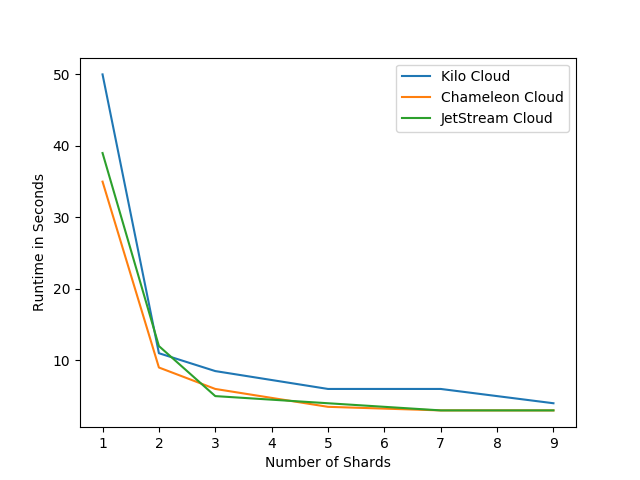
\includegraphics[width=\linewidth]{../project/S17-IO-3012/report/images/shard_find.png}}
\caption{Find Command - Sharding Test}
\label{fig:shard-find}
\end{figure}


All three clouds show a particularly large gain in performance when in
increasing from one shard to two.  Run time for two shards is less
than one third the run time of one shard.  Increases in shards beyond
two show much smaller incremental gains.

Perfomance on Chameleon Cloud and Jetstream is very similar for the
find test.  Kilo performance is worse, although proportunately better
than on the mongoimport test.  This is an interesting observation as
for both deployment and mongoimport, performance was much better on
Chameleon and Futuresystems than Kilo.  One difference from the
mongoimport test is that much less data is being sent over the
network.  Network speeds could be a factor in this discrepancy.


\subsubsection{Impact of Sharding on Writes}




Figure \ref{fig:shard-import} depicts the impact on performance of
various numbers of shards on a mongoimport command in the three
clouds.  For all clouds, run time of the mongoimport command in our
tests does not appear to be impacted by the number of shards.  Since
the same amount of data is written with more computing resources
available when there are more shards, we might expect to see a
performance gain.  However, there are possible explanations for
performance not improving.  First, the mongoimport command may not
write data in parallel.  This is not indicated in the documentation,
but it seems likely that it reads the file serially.  Second,
resources on the server the data is written to may not be the
bottleneck in the write process.  Other resources like the network
time seem more likely to be the bottleneck.  Since we are always going
over the network from the mongos instance to a data shard, regardless
of the number of shards, a bottleneck in the network would impact all
shard configurations equally.

\begin{figure}[htbp]
\centering
\fbox{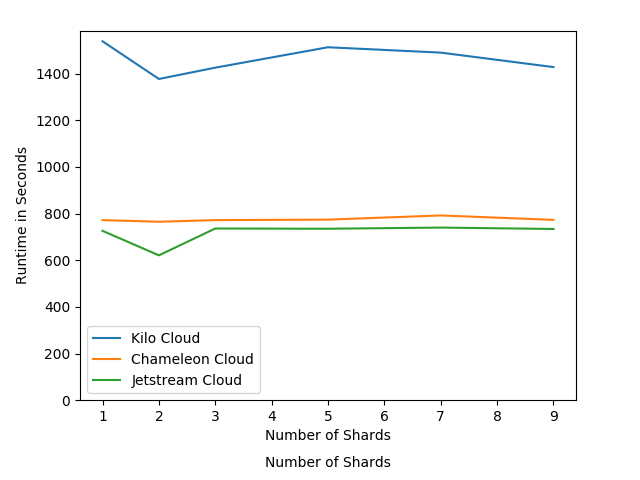
\includegraphics[width=\linewidth]{../project/S17-IO-3012/report/images/shard_import.png}}
\caption{Mongoimport Command - Sharding Test}
\label{fig:shard-import}
\end{figure}

While sharding did not benefit a single threaded mongoimport command,
it is likely it would benefit other heavy write operations,
particularly coming through multiple mongos instances.  In a
non-sharded environment, this would lead to a heavy load on the single
data shard.  In a sharded environment, the load on each shard would
drop as the number of shards increased.

While performance on Chameleon and FutureSystems was very similar for
the find command, performance of the mongoimport command was
significantly better on Chameleon than on Kilo.  We see approximately
50\% better performance on both Chameleon and Jetstream Clouds
compared to FutureSystems. Jetstream performance is slightly better
than Chameleon for the import test.


\subsubsection{Impact of Sharding on MapReduce}



Figure \ref{fig:shard-mapreduce} shows the performance of MapReduce
across varous sharding configurations on our three clouds.  These
results are relatively similar to the find results.  While results are
inconsistent, particularly on Futuresystems, likely due to
environmental issues, all clouds show an overall decrease in
processing time with addition of shards.  Relative to Mongoimport
performance, performance is more similar across the three clouds for
MapReduce.

\begin{figure}[htbp]
\centering
\fbox{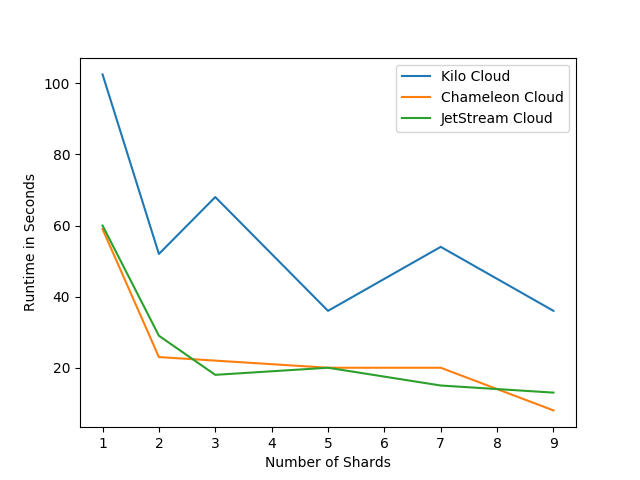
\includegraphics[width=\linewidth]{../project/S17-IO-3012/report/images/shard_mapreduce.png}}
\caption{MapReduce - Sharding Test}
\label{fig:shard-mapreduce}
\end{figure}


\subsubsection{Impact of Replication on Reads}



Figure \ref{fig:replica-find} depicts the impact on performance of
various numbers of replicas on a find command in Chameleon,
FutureSystems, and Jetstream Clouds.  These results show no
correlation between the number of replicas and find performance.

\begin{figure}[htbp]
\centering
\fbox{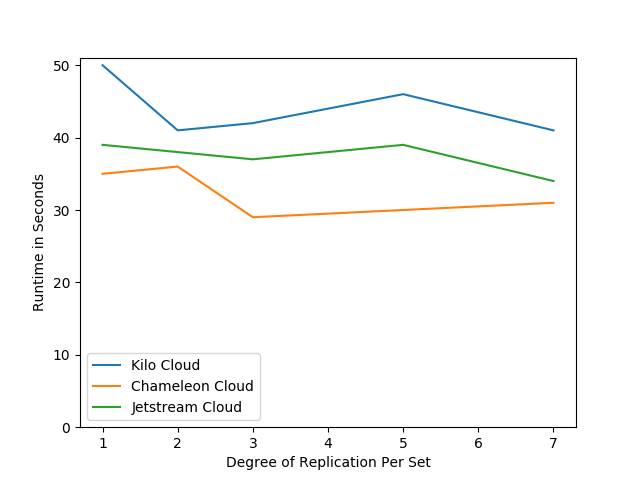
\includegraphics[width=\linewidth]{../project/S17-IO-3012/report/images/replica_find.png}}
\caption{Find Command - Replication Test}
\label{fig:replica-find}
\end{figure}

Similarly to other tests, performance on Chameleon was best for the
majority of the test runs in the find replication test, followed by
Jetstream, with Futuresystems performing the worst.


\subsubsection{Impact of Replication on Writes}


\begin{figure}[htbp]
\centering
\fbox{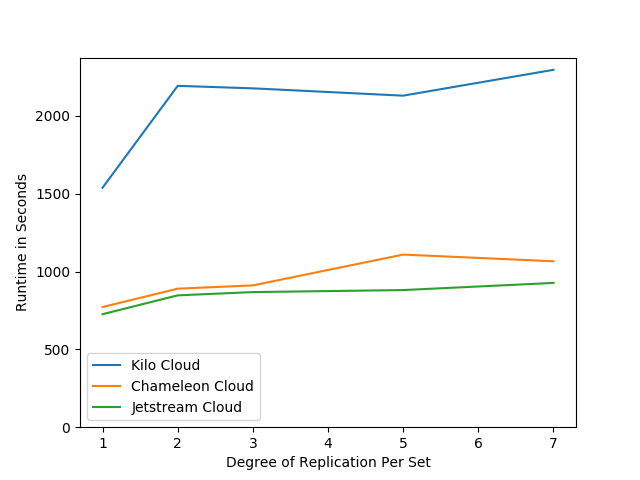
\includegraphics[width=\linewidth]{../project/S17-IO-3012/report/images/replica_import.png}}
\caption{Mongoimport Command - Replication Test}
\label{fig:replica-import}
\end{figure}


Figure \ref{fig:replica-import} depicts the impact on performance of
various numbers of replicas on a mongoimport command on our three
Clouds.  The results show poorer write performance as the number of
replicas increase.  Given that an extra copy of data is written with
each increase in the replication factor, this performance hit is
expected.

Performance on Jetstream and Chameleon were very close on this test
with Chameleon only performing significantly better with four or more
replicas.  FutureSystems import performance was by far the worst of
the three clouds.


\subsubsection{Impact of Replication on MapReduce}

\begin{figure}[htbp]
\centering
\fbox{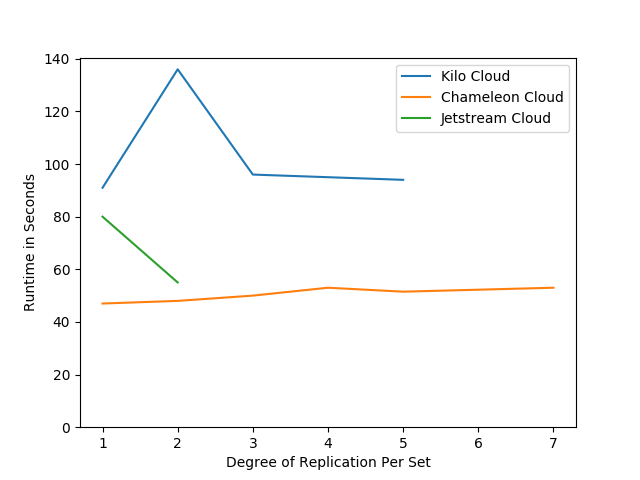
\includegraphics[width=\linewidth]{../project/S17-IO-3012/report/images/replica_mapreduce.png}}
\caption{MapReduce - Replication Test}
\label{fig:replica-mapreduce}
\end{figure}

As shown in Figure \ref{fig:replica-mapreduce}, replication appears to
have no impact on MapReduce operations.  While there are variations in
FutureSystems and Jetstream performance for different numbers of
replicas, they do not follow a consistent pattern and appear to be
caused by environmental issues.  This is an interesting result as
increased levels of replication came with a performance penalty for
the find commmand, which also reads data.

As with several other tests, Chameleon MapReduce performance was the
best, followed by Jetstream, with FutureSystems again being the worst.


\subsubsection{Impact of Version and Sharding on Reads}


\begin{figure}[htbp]
\centering
\fbox{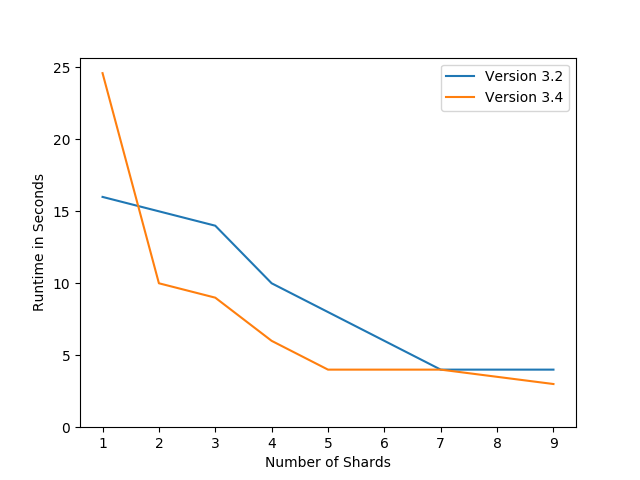
\includegraphics[width=\linewidth]{../project/S17-IO-3012/report/images/version_find.png}}
\caption{Find Command - Version 3.2 vs 3.4}
\label{fig:version-find}
\end{figure}

Figure \ref{fig:version-find} shows the MongoDB version 3.4 and 3.2
find performance on Chameleon Cloud.  Results are very close, with
version 3.2 having the best performance for one shard and performance
being similar for all other sharding levels.

\subsubsection{Impact of Version and Sharding on Writes}

\begin{figure}[htbp]
\centering
\fbox{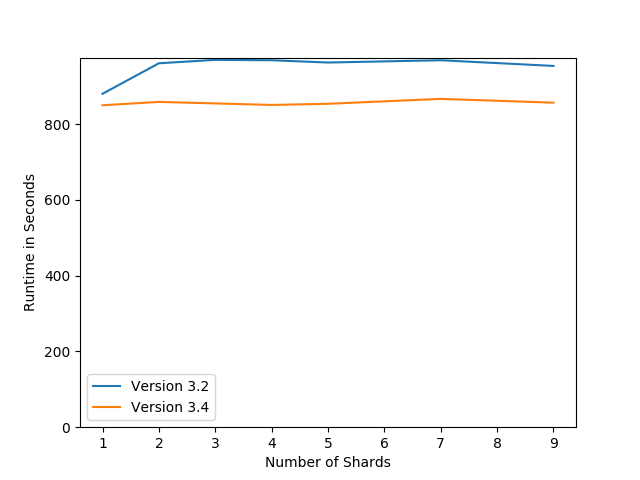
\includegraphics[width=\linewidth]{../project/S17-IO-3012/report/images/version_import.png}}
\caption{Mongoimport Command - Version 3.2 vs 3.4}
\label{fig:version-import}
\end{figure}


Figure \ref{fig:version-import} shows the MongoDB version 3.4 and 3.2
Mongoimport performance on Chameleon Cloud. Runtimes are similar for
each version.  Version 3.2 is slightly faster at the lowest sharding
levels and Version 3.4 is slightly faster at the highest sharding
level.  Given the mixed results and close run times, neither version
shows a significant advantage for write operations.


\subsubsection{Impact of Version and Sharding on MapReduce}

Figure \ref{fig:version-mapreduce} shows the MongoDB version 3.4 and
3.2 Mongoimport performance on Chameleon Cloud.  Runtimes are similar
for each version and with each version being faster at some shard
level, which appears to be random. Given the mixed results and close
run times, neither version shows a significant advantage for MapReduce
operations.

\begin{figure}[htbp]
\centering
\fbox{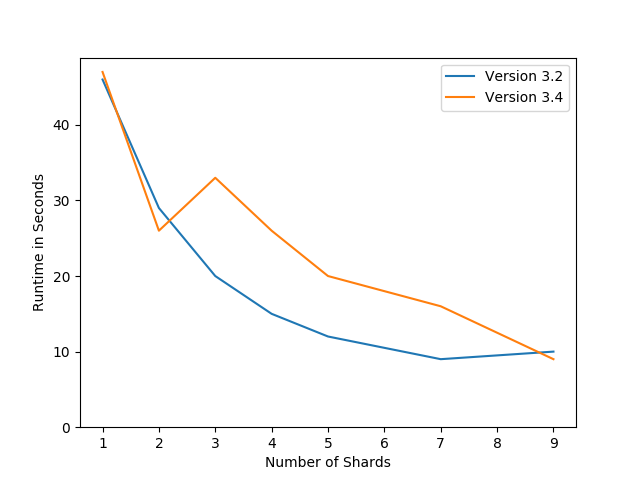
\includegraphics[width=\linewidth]{../project/S17-IO-3012/report/images/version_mapreduce.png}}
\caption{MapReduce - Version 3.2 vs 3.4}
\label{fig:version-mapreduce}
\end{figure}

\section{Conclusion}

We have created, tested, and demonstrated a fully automated program to
configure and deploy a sharded MongoDB clus- ter to three cloud
environments: Chameleon, Jetstream, and FutureSystems. Using a
combination of Python, Bash, and Cloudmesh Client, the a cluster is
dynamically deployed with a selected number of Config Server Replicas,
Mongos Routers, Shards, and Shard Replicas and either MongoDB version
3.4 or 3.2. Functions also exist for terminating the environment,
reporting on data distribution, benchmarking, and reporting on
performance testing.  An automated benchmarking process to show the
impact of well distributed data across shards of a large data set has
been run for various configurations. The impact of MongoDB ver- sion
3.4 versus 3.2, Sharding, and Replication on performance have been
assessed. Testing showed performance and stability on Chameleon Cloud
to be the best of our three cloud environ- ments with Jetstream a
close second after an operational issue was resolved by the support
team. Futuresystems performance consistently lagged behind the other
two clouds due to its older hardware. A key finding is that read
performance, typically a high priority for noSQL data stores and Big
Data operations, increases significantly as shards are added. Testing
also showed that a predictable performance penalty is associated with
replication. Our comparison of version 3.4 and 3.2 showed no
significant differences between version 3.2 and 3.4 performance across
various sharding levels.



\bibliographystyle{ACM-Reference-Format}
\bibliography{references} 

\end{document}

